\section{Arquiteturas}

Esse capítulo apresenta diversas arquiteturas possíveis através do 
protocolo OpenFlow. 
O protocolo foi desenvolvido de uma maneira bem aberta para que pudesse 
compreender diversas topologias de rede. 

\subsection{Topologia simples}

Uma topologia simples pode ser vista na figura \ref{fig:simple-topology} onde
um controlador manipula o plano de dados através de um switch OpenFlow 
que possui 3 computadores (\emph{hosts}).

\begin{figure}[h!]
    \centering
    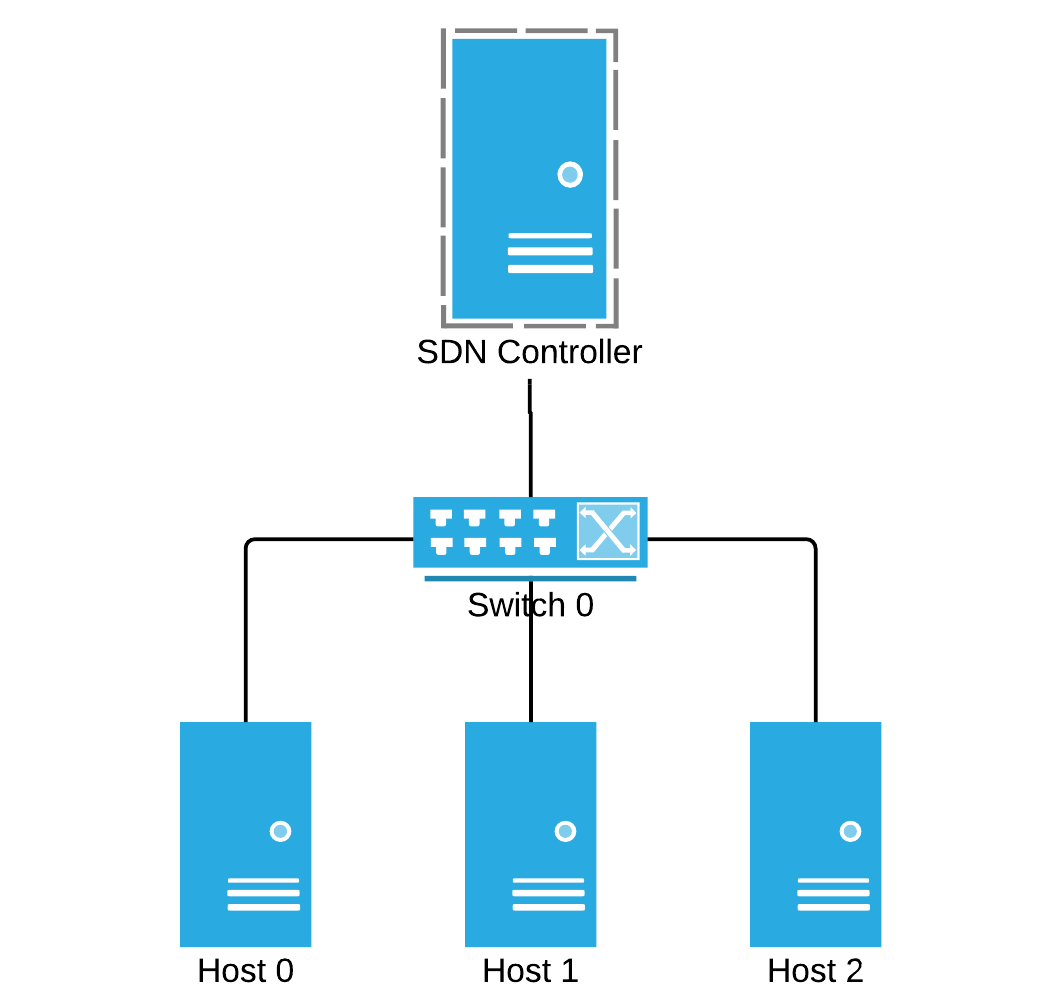
\includegraphics{img/simple-topology}
    \label{fig:simple-topology}
    \caption{Topologia simples de redes de computadores}
\end{figure}


\subsection{Um controlador para \emph{n} switches}

\subsection{\emph{n} Controladores para \emph{n} switches}

\subsection{Controlador distribuído}

\subsection{Arquitetura para a Internet}
